% Options for packages loaded elsewhere
\PassOptionsToPackage{unicode}{hyperref}
\PassOptionsToPackage{hyphens}{url}
%
\documentclass[
  openany]{book}
\usepackage{lmodern}
\usepackage{amssymb,amsmath}
\usepackage{ifxetex,ifluatex}
\ifnum 0\ifxetex 1\fi\ifluatex 1\fi=0 % if pdftex
  \usepackage[T1]{fontenc}
  \usepackage[utf8]{inputenc}
  \usepackage{textcomp} % provide euro and other symbols
\else % if luatex or xetex
  \usepackage{unicode-math}
  \defaultfontfeatures{Scale=MatchLowercase}
  \defaultfontfeatures[\rmfamily]{Ligatures=TeX,Scale=1}
\fi
% Use upquote if available, for straight quotes in verbatim environments
\IfFileExists{upquote.sty}{\usepackage{upquote}}{}
\IfFileExists{microtype.sty}{% use microtype if available
  \usepackage[]{microtype}
  \UseMicrotypeSet[protrusion]{basicmath} % disable protrusion for tt fonts
}{}
\makeatletter
\@ifundefined{KOMAClassName}{% if non-KOMA class
  \IfFileExists{parskip.sty}{%
    \usepackage{parskip}
  }{% else
    \setlength{\parindent}{0pt}
    \setlength{\parskip}{6pt plus 2pt minus 1pt}}
}{% if KOMA class
  \KOMAoptions{parskip=half}}
\makeatother
\usepackage{xcolor}
\IfFileExists{xurl.sty}{\usepackage{xurl}}{} % add URL line breaks if available
\IfFileExists{bookmark.sty}{\usepackage{bookmark}}{\usepackage{hyperref}}
\hypersetup{
  pdfauthor={My Name},
  hidelinks,
  pdfcreator={LaTeX via pandoc}}
\urlstyle{same} % disable monospaced font for URLs
\usepackage[margin=1in]{geometry}
\usepackage{color}
\usepackage{fancyvrb}
\newcommand{\VerbBar}{|}
\newcommand{\VERB}{\Verb[commandchars=\\\{\}]}
\DefineVerbatimEnvironment{Highlighting}{Verbatim}{commandchars=\\\{\}}
% Add ',fontsize=\small' for more characters per line
\usepackage{framed}
\definecolor{shadecolor}{RGB}{248,248,248}
\newenvironment{Shaded}{\begin{snugshade}}{\end{snugshade}}
\newcommand{\AlertTok}[1]{\textcolor[rgb]{0.94,0.16,0.16}{#1}}
\newcommand{\AnnotationTok}[1]{\textcolor[rgb]{0.56,0.35,0.01}{\textbf{\textit{#1}}}}
\newcommand{\AttributeTok}[1]{\textcolor[rgb]{0.77,0.63,0.00}{#1}}
\newcommand{\BaseNTok}[1]{\textcolor[rgb]{0.00,0.00,0.81}{#1}}
\newcommand{\BuiltInTok}[1]{#1}
\newcommand{\CharTok}[1]{\textcolor[rgb]{0.31,0.60,0.02}{#1}}
\newcommand{\CommentTok}[1]{\textcolor[rgb]{0.56,0.35,0.01}{\textit{#1}}}
\newcommand{\CommentVarTok}[1]{\textcolor[rgb]{0.56,0.35,0.01}{\textbf{\textit{#1}}}}
\newcommand{\ConstantTok}[1]{\textcolor[rgb]{0.00,0.00,0.00}{#1}}
\newcommand{\ControlFlowTok}[1]{\textcolor[rgb]{0.13,0.29,0.53}{\textbf{#1}}}
\newcommand{\DataTypeTok}[1]{\textcolor[rgb]{0.13,0.29,0.53}{#1}}
\newcommand{\DecValTok}[1]{\textcolor[rgb]{0.00,0.00,0.81}{#1}}
\newcommand{\DocumentationTok}[1]{\textcolor[rgb]{0.56,0.35,0.01}{\textbf{\textit{#1}}}}
\newcommand{\ErrorTok}[1]{\textcolor[rgb]{0.64,0.00,0.00}{\textbf{#1}}}
\newcommand{\ExtensionTok}[1]{#1}
\newcommand{\FloatTok}[1]{\textcolor[rgb]{0.00,0.00,0.81}{#1}}
\newcommand{\FunctionTok}[1]{\textcolor[rgb]{0.00,0.00,0.00}{#1}}
\newcommand{\ImportTok}[1]{#1}
\newcommand{\InformationTok}[1]{\textcolor[rgb]{0.56,0.35,0.01}{\textbf{\textit{#1}}}}
\newcommand{\KeywordTok}[1]{\textcolor[rgb]{0.13,0.29,0.53}{\textbf{#1}}}
\newcommand{\NormalTok}[1]{#1}
\newcommand{\OperatorTok}[1]{\textcolor[rgb]{0.81,0.36,0.00}{\textbf{#1}}}
\newcommand{\OtherTok}[1]{\textcolor[rgb]{0.56,0.35,0.01}{#1}}
\newcommand{\PreprocessorTok}[1]{\textcolor[rgb]{0.56,0.35,0.01}{\textit{#1}}}
\newcommand{\RegionMarkerTok}[1]{#1}
\newcommand{\SpecialCharTok}[1]{\textcolor[rgb]{0.00,0.00,0.00}{#1}}
\newcommand{\SpecialStringTok}[1]{\textcolor[rgb]{0.31,0.60,0.02}{#1}}
\newcommand{\StringTok}[1]{\textcolor[rgb]{0.31,0.60,0.02}{#1}}
\newcommand{\VariableTok}[1]{\textcolor[rgb]{0.00,0.00,0.00}{#1}}
\newcommand{\VerbatimStringTok}[1]{\textcolor[rgb]{0.31,0.60,0.02}{#1}}
\newcommand{\WarningTok}[1]{\textcolor[rgb]{0.56,0.35,0.01}{\textbf{\textit{#1}}}}
\usepackage{longtable,booktabs}
% Correct order of tables after \paragraph or \subparagraph
\usepackage{etoolbox}
\makeatletter
\patchcmd\longtable{\par}{\if@noskipsec\mbox{}\fi\par}{}{}
\makeatother
% Allow footnotes in longtable head/foot
\IfFileExists{footnotehyper.sty}{\usepackage{footnotehyper}}{\usepackage{footnote}}
\makesavenoteenv{longtable}
\usepackage{graphicx,grffile}
\makeatletter
\def\maxwidth{\ifdim\Gin@nat@width>\linewidth\linewidth\else\Gin@nat@width\fi}
\def\maxheight{\ifdim\Gin@nat@height>\textheight\textheight\else\Gin@nat@height\fi}
\makeatother
% Scale images if necessary, so that they will not overflow the page
% margins by default, and it is still possible to overwrite the defaults
% using explicit options in \includegraphics[width, height, ...]{}
\setkeys{Gin}{width=\maxwidth,height=\maxheight,keepaspectratio}
% Set default figure placement to htbp
\makeatletter
\def\fps@figure{htbp}
\makeatother
\setlength{\emergencystretch}{3em} % prevent overfull lines
\providecommand{\tightlist}{%
  \setlength{\itemsep}{0pt}\setlength{\parskip}{0pt}}
\setcounter{secnumdepth}{5}
\usepackage[none]{hyphenat}
\pagestyle{plain}
\raggedbottom
\usepackage{hyperref}
\usepackage{floatpag}
\floatpagestyle{empty}
\usepackage{booktabs}
\usepackage{float}
\usepackage[document]{ragged2e} % left-justified text - comment for fully justified text
\usepackage{nonumonpart}

% define abstract environment
\newcommand\abstractname{Abstract}

\makeatletter
 \if@titlepage
  \newenvironment{abstract}{%
      \titlepage
      \null\vfil
      \@beginparpenalty\@lowpenalty
      \begin{center}%
        \bfseries \abstractname
        \@endparpenalty\@M
      \end{center}}%
     {\par\vfil\null\endtitlepage}
\else
  \newenvironment{abstract}{%
      \if@twocolumn
        \section*{\abstractname}%
      \else
        \small
        \begin{center}%
          {\bfseries \abstractname\vspace{-.5em}\vspace{\z@}}%
        \end{center}%
        \quotation
      \fi}
      {\if@twocolumn\else\endquotation\fi}
\fi
\makeatother

\frontmatter
% https://github.com/rstudio/rmarkdown/issues/337
\let\rmarkdownfootnote\footnote%
\def\footnote{\protect\rmarkdownfootnote}

% https://github.com/rstudio/rmarkdown/pull/252
\usepackage{titling}
\setlength{\droptitle}{-2em}

\pretitle{\vspace{\droptitle}\centering\huge}
\posttitle{\par}

\preauthor{\centering\large\emph}
\postauthor{\par}

\predate{\centering\large\emph}
\postdate{\par}

\author{My Name}
\date{2019}

\begin{document}
\frontmatter

\begin{titlepage}
\begin{center}
\vspace*{5cm}
\Huge{\textbf{Thesis Title}}

\vspace*{3cm}
\Large{Thesis Subtitle}
\vfill
\Large{\textbf{Author Name}}
\vfill
Dissertation for MSc Data Science

\vspace{0.8cm}

\includegraphics[width=0.4\textwidth]{img/lu-logo-cmyk.jpg}

School of Computing and Communications\\
Lancaster University\\
Lancaster, UK\\
\today
\end{center}
\end{titlepage}


\thispagestyle{empty}


\begin{abstract}
My abstract goes here...
\end{abstract}

\newpage

\chapter*{Preface}

Thanks goes to.

\setcounter{page}{1}

{
\setcounter{tocdepth}{1}
\tableofcontents
}
\listoftables
\listoffigures
\mainmatter
\hypertarget{introduction}{%
\chapter{Introduction}\label{introduction}}

\hypertarget{background-information}{%
\section{Background information}\label{background-information}}

\begin{itemize}
\tightlist
\item
  text 1
\item
  text 2
\item
  text 3
\item
  more text
\item
  more text
\end{itemize}

\hypertarget{literature-review}{%
\section{Literature review}\label{literature-review}}

One important development was made by Abrams, Gillies, and Lambert (\protect\hyperlink{ref-Abrams2005}{2005}).

\hypertarget{methods}{%
\chapter{Methods}\label{methods}}

\hypertarget{important-main-method}{%
\section{Important main method}\label{important-main-method}}

Initial modelling was performed using linear regression as defined in equation \eqref{eq:linreg}.

\begin{equation}
y_i = \beta_0 + \beta_1x_i + \varepsilon_i,\  \varepsilon_i \overset{iid}{\sim} N(0, \sigma^2)
\label{eq:linreg}
\end{equation}

\hypertarget{additional-method}{%
\section{Additional method}\label{additional-method}}

\begin{itemize}
\tightlist
\item
  text 6
\item
  text 7
\end{itemize}

\hypertarget{results}{%
\chapter{Results}\label{results}}

\hypertarget{main-results}{%
\section{Main results}\label{main-results}}

And here is an example table of regression coefficients in Table \ref{tab:mtreg}.

\begin{Shaded}
\begin{Highlighting}[]
\NormalTok{mod <-}\StringTok{ }\KeywordTok{lm}\NormalTok{(mpg }\OperatorTok{~}\StringTok{ }\NormalTok{wt, }\DataTypeTok{data =}\NormalTok{ mtcars)}
\NormalTok{coefcis <-}\StringTok{ }\KeywordTok{cbind}\NormalTok{(}\KeywordTok{coef}\NormalTok{(mod), }\KeywordTok{confint.default}\NormalTok{(mod))}
\KeywordTok{colnames}\NormalTok{(coefcis) <-}
\StringTok{  }\KeywordTok{c}\NormalTok{(}\StringTok{"Estimate"}\NormalTok{, }\StringTok{"95% CI lower limit"}\NormalTok{, }\StringTok{"95% CI upper limit"}\NormalTok{)}
\NormalTok{knitr}\OperatorTok{::}\KeywordTok{kable}\NormalTok{(coefcis,}
             \DataTypeTok{digits =} \DecValTok{2}\NormalTok{,}
             \DataTypeTok{booktabs =} \OtherTok{TRUE}\NormalTok{,}
             \DataTypeTok{caption =} \StringTok{"Parameter estimates from regression of mpg on weight."}\NormalTok{) }\OperatorTok
\StringTok{  }\KeywordTok{kable_styling}\NormalTok{(}\DataTypeTok{latex_options =} \KeywordTok{c}\NormalTok{(}\StringTok{"HOLD_position"}\NormalTok{))}
\end{Highlighting}
\end{Shaded}

\begin{table}[H]

\caption{\label{tab:mtreg}Parameter estimates from regression of mpg on weight.}
\centering
\begin{tabular}[t]{lrrr}
\toprule
  & Estimate & 95\% CI lower limit & 95\% CI upper limit\\
\midrule
(Intercept) & 37.29 & 33.61 & 40.97\\
wt & -5.34 & -6.44 & -4.25\\
\bottomrule
\end{tabular}
\end{table}

Example text example text example text example text example text example text example text example text example text example text example text example text example text example text example text example text example text example text.

An example of a figure is shown in Figure \ref{fig:pressure}.

\begin{Shaded}
\begin{Highlighting}[]
\KeywordTok{plot}\NormalTok{(pressure, }\DataTypeTok{pch =} \DecValTok{19}\NormalTok{, }\DataTypeTok{type =} \StringTok{"b"}\NormalTok{)}
\end{Highlighting}
\end{Shaded}

\begin{figure}[H]

{\centering 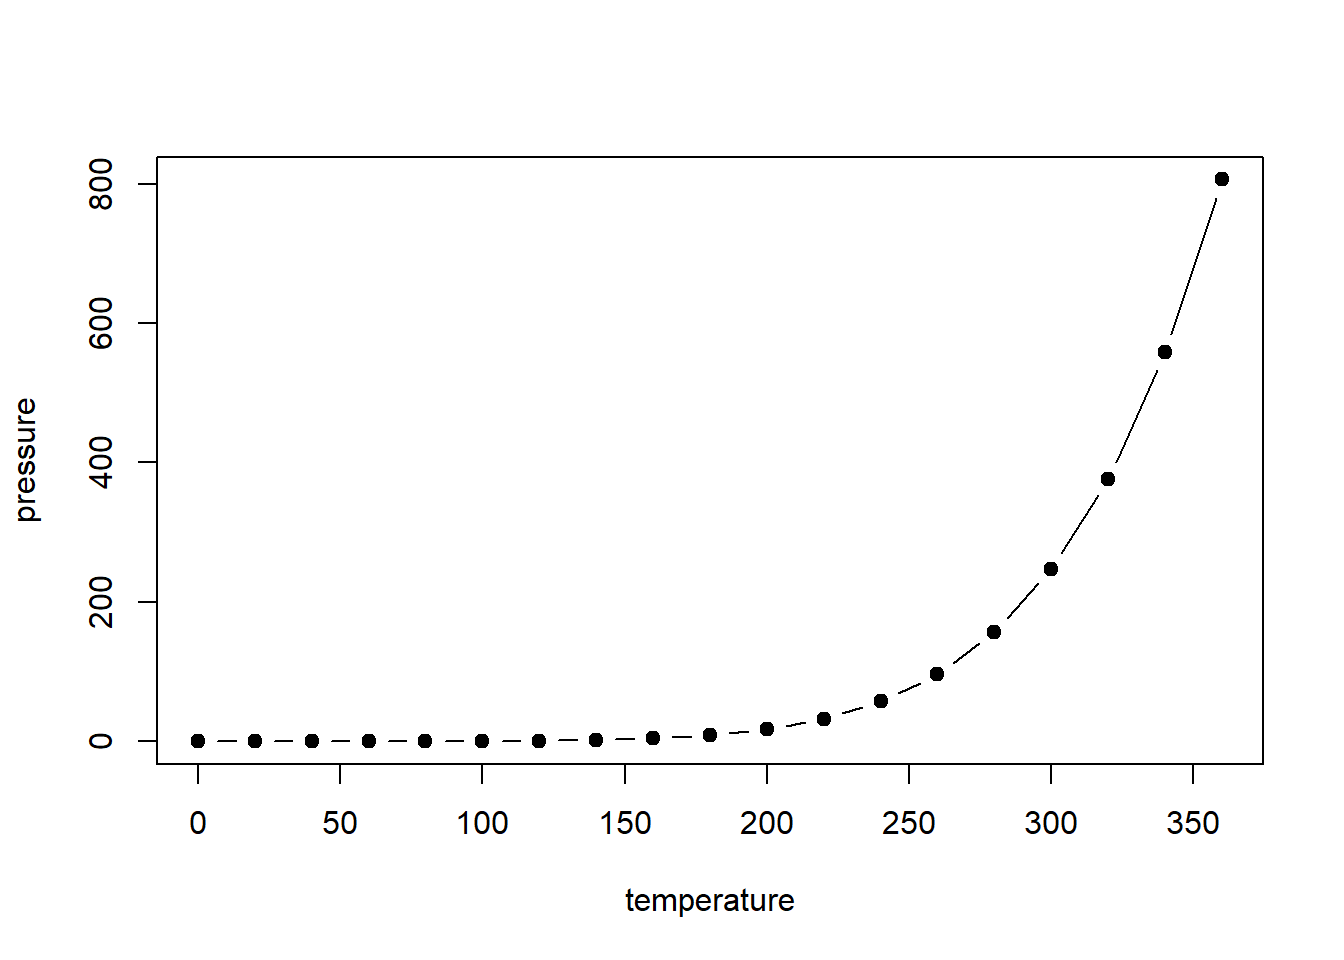
\includegraphics[width=0.75\linewidth]{03_results_files/figure-latex/pressure-1} 

}

\caption{An example figure.}\label{fig:pressure}
\end{figure}

And we can include image files directly, such as Figure \ref{fig:knitlogo}.

\begin{Shaded}
\begin{Highlighting}[]
\NormalTok{knitr}\OperatorTok{::}\KeywordTok{include_graphics}\NormalTok{(}\StringTok{"img/mtcars-scatter.png"}\NormalTok{)}
\end{Highlighting}
\end{Shaded}

\begin{figure}

{\centering 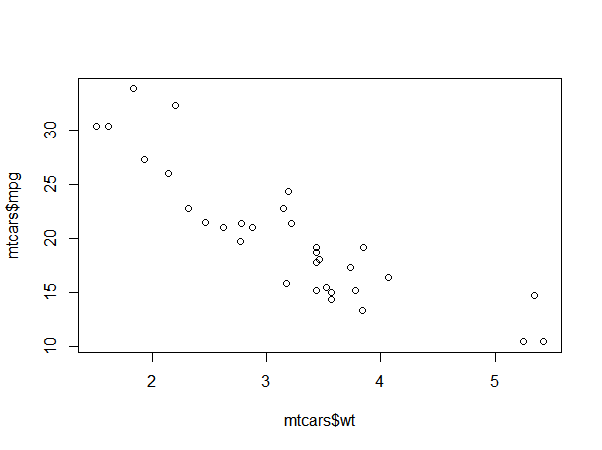
\includegraphics[width=0.75\linewidth]{img/mtcars-scatter} 

}

\caption{Another example figure.}\label{fig:knitlogo}
\end{figure}

To figure code chunks add the chunk option \texttt{fig.pos="H"} to use the LaTeX float package to try and position the figure where the code appears.

Also, this is how to reference a section, e.g.~the Introduction was chapter \ref{introduction} and the Literature Review was section \ref{literature-review}.

\hypertarget{discussion}{%
\chapter{Discussion}\label{discussion}}

\hypertarget{what-i-found}{%
\section{What I found}\label{what-i-found}}

\begin{itemize}
\tightlist
\item
  text 1
\item
  text 2
\item
  text 3
\item
  more text
\item
  more text
\end{itemize}

\hypertarget{what-it-means}{%
\section{What it means}\label{what-it-means}}

\begin{itemize}
\tightlist
\item
  text 6
\item
  text 7
\end{itemize}

\hypertarget{references}{%
\chapter{References}\label{references}}

\hypertarget{refs}{}
\leavevmode\hypertarget{ref-Abrams2005}{}%
Abrams, K. R., C. L. Gillies, and P. C. Lambert. 2005. ``Meta-Analysis of Heterogeneously Reported Trials Assessing Change from Baseline.'' \emph{Statistics in Medicine} 24: 3823--44.

\hypertarget{appendix-appendix}{%
\appendix}


\hypertarget{appendix-of-r-code}{%
\chapter*{Appendix of R code}\label{appendix-of-r-code}}
\addcontentsline{toc}{chapter}{Appendix of R code}

\begin{Shaded}
\begin{Highlighting}[]
\NormalTok{model <-}\StringTok{ }\KeywordTok{lm}\NormalTok{(y }\OperatorTok{~}\StringTok{ }\NormalTok{x1 }\OperatorTok{+}\StringTok{ }\NormalTok{x2, }\DataTypeTok{data =}\NormalTok{ df)}
\KeywordTok{summary}\NormalTok{(model)}
\end{Highlighting}
\end{Shaded}

\backmatter
\backmatter

\end{document}
